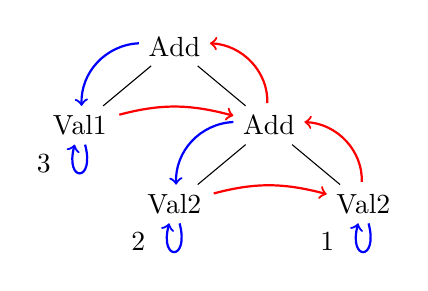
\begin{tikzpicture}
  % \tikzstyle{every node}=[font=\footnotesize]
  \tikzstyle{level 1}=[level distance=10mm, sibling distance=24mm]
  \tikzstyle{level 2}=[level distance=10mm, sibling distance=24mm]
  \tikzstyle{level 3}=[level distance=10mm, sibling distance=14mm]
  \tikzstyle{load}=[->,thick,color=blue]
  \tikzstyle{unload}=[->,shorten <=1pt,thick,color=red]

  \node (root) {\AI{Add}}
    child {node (node1) [label=below left:\pgftextcircled{3}] {\AI{Val}\AS{}\AN{1}}} 
    child {node (node2) {\AI{Add}} 
           child {node (node3) [label=below left:\pgftextcircled{2}] {\AI{Val}\AS{}\AN{2}}}
           child {node (node4) [label=below left:\pgftextcircled{1}] {\AI{Val}\AS{}\AN{2}}}};


  {\draw[load] (root) to [ bend right=45] (node1);}
  {\draw[load] (node1) to [ loop below ] (node1);}
  {\draw[unload] (node1) to [ bend left=15] (node2);}
  {\draw[load] (node2) to [ bend right=45] (node3);}
  {\draw[load] (node3) to [ loop below] (node3);}
  {\draw[unload] (node3) to [ bend left=15] (node4);}
  {\draw[load] (node4) to [ loop below] (node4);}
  {\draw[unload] (node4) to [ bend right=45] (node2);}
  {\draw[unload] (node2) to [ bend right=45] (root);}
\end{tikzpicture}
